\documentclass[a4paper, 12pt]{article}
\usepackage[T1]{fontenc}
\usepackage[margin=1in]{geometry}
\usepackage{indentfirst}
\usepackage{enumitem}
\usepackage{graphicx}
\usepackage{lipsum}
\usepackage{float}
\usepackage[most]{tcolorbox}
\usepackage{media9}
\usepackage{hyperref}

\hypersetup{
    colorlinks=true,
    linkcolor=blue,
    urlcolor=cyan,
}

\definecolor{shadecolor}{gray}{0.9}
\newtcolorbox{example}{colback=shadecolor,grow to right by=-30pt,grow to left by=-30pt,breakable,adjusted title={Example}}

\newcommand{\Example}[1]{\begin{example}#1\end{example}}

\begin{document}
\title{HESS - CRSR - Automarker (Amongsus) Report}
\author{Vivan Waghela \and Ayush Acharjya \and Ye Aung (James) \and Selahattin Satilmis}
\date{7th December 2024}
\maketitle

\section*{DEMO VIDEO}
\subsection*{Only works in latest versions of Adobe Acrobat and Okular PDF}
\noindent\href{run:demo.mp4}{Video Link}

\vspace{3mm}

\noindent\includemedia[
  width=\textwidth,
  addresource=demo.mp4,
  flashvars={source=demo.mp4}
]{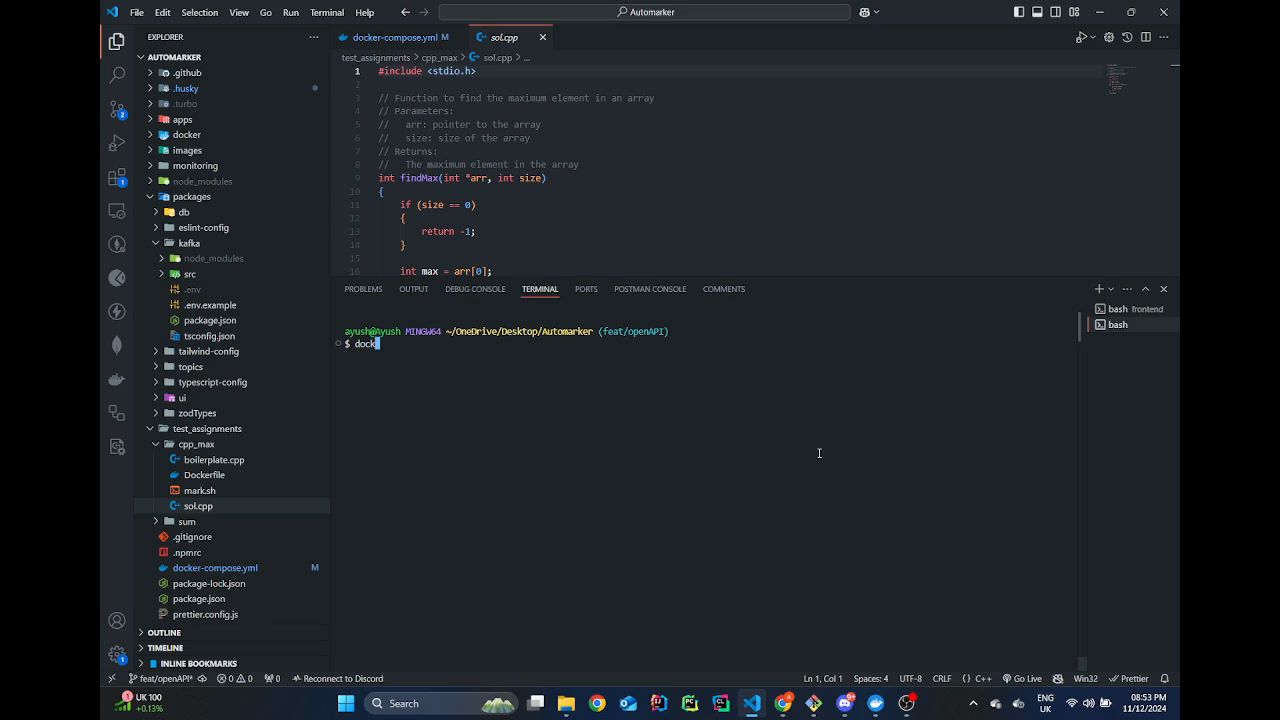
\includegraphics[width=\textwidth]{thumbnail.png}}{VPlayer.swf}

\section*{Link to the online repository}
\noindent\url{https://github.com/Ayush272002/Automarker}

\section*{Summary}
We decided to use Ayush's EDR for our prototype. As Module Organisers could need more customisability than pre-built containers, we changed our prototype to allow them to upload a Dockerfile along with a test file that would be executed inside the docker container. We were able to make a working version of the auto-marking system described in the EDR. The system is able to run the submitted programming assignment against tests defined in test file. The markers can customise the test file as much as they like. The system also reduces human error as the code will be executed and the marks will be calculated based on the output of the test file. As per non-functional requirements, we were able to allow our system to mark code for any possible programming language (as long as there is a way to mark it with a shell file and a Dockerfile). As the CSRS product has an open API for developers to use, we included our submission API in the existing open API so that technically-savy users can automate parts of submission.

\section*{Accomplishments}
To keep track of the development process, we decided to use GitHub Issues (see Fig.~\ref{fig:issues}). We also used Discord to communicate with each other, including weekly meetings, general calls to help each other and keep track of what is being updated in the repository, etc, and we took detailed meeting notes every meeting. To make sure our code works before it is merged into the main branch, we first individually tested our code by simply running it, then a pre-commit hook makes sure the code builds before a commit is made. Once the pre-commit hook succeeds, we would create a Pull Request for the feature being made. The repository restricts merging until a reviewer other than themself approves it, and requires that the CI check passes. Once merged, our CD pipeline builds the backend and engine docker images and pushes it into the dockerhub and verifies that it has been pushed. The CI pipeline also runs after a merge occurs into the main branch to make sure the merged code does not fail any tests.

\subsection*{Project Management}
We implemented the Agile development strategy, which was easiest for our team to work with as implementing a system like our prototype can and will have bugs that we would potentially run into during development.

In our first meeting for this project, we decided that Vivan would work mainly on the backend, Ayush would work mainly on the engine, devops, and some parts of the backend, James would work mainly on the student frontend, and Selahattin would work mainly on the marker frontend. Since James and Selahattin worked mainly on parts of the frontend, they also worked on the UX for the website. During development, James and Selahattin had a lot of questions, so Vivan and Ayush collaborated with them throughout the frontend development process.

Many times, the frotnend team needed to communicate with the backend team about what the backend would return in specific API routes. Sometimes, team members had written entire features including frontend and backend parts. This would be communicated beforehand so that other group members would not be confused. This would lead to many parts of each of the system being completed quicker as more features would be implemented at the same time.

\subsection*{Planning}
Throughout the entire project, each member was transparent on what work they finished, what they need to finish, and what they needed help with. We also set deadlines so that each feature would be completed and tested thouroughly on time. There were times that a feature was not finished by a deadline due to complex errors that had to be debugged multiple times by other group members.

\Example {There was an issue where the CI pipeline could not build the project as it was reporting a very generic error, however, it was successfully building on all machines within the group. After doing tons of research, we found that we simply needed to add an optional dependency in the \emph{package.json} file}

As per our planning, we finished the project 2 days before the dealine of the prototype, all thanks to our planning that allowed deadlines to be moved whenever needed. We used the remaining time to polish the project by cleaning up some of the code and increase the project's efficiency.

Like any group, we also had a few miscommunications that occurred throughout the development process:

\Example {In the beginning of the project, one of our group members decided to use MUI as the components library without informing the others. However, in our first meeting, we had decided to use shadcn as our components library. In the next meeting, we discussed if we should continue to use shadcn or if we should switch to MUI for our components library. In the end, we decided to stick to shadcn.}
         
There were also times where two teammates had different ways a problem could be fixed, and both preferred their own fix. To resolve this conflict, we would have a meeting that would attempt to find a middleground. We would discuss the pros and cons of each approach, and we would try and merge both solutions to include as many pros from both approaches and leave out as many cons from both approaches.

\subsection*{Technical Achievments}
We decided to use a monorepo for our project as we knew there would be shared code which would implement the DRY coding practice. Our frontend used NextJS, our backend used ExpressJS, and our engine (microservice) uses NodeJS. We used Kafka for our async communication system. All systems were implemented in Typescript. We also used Storybook to individually test our components in isolation.

We built our prototype to be very scalable, which is why our prototype uses a microservice-based system architecture (see Fig.~\ref{fig:system-architecture}). We used Prometheus and Grafana to monitor our backend API services. We also included an OpenAPI spec in our backend to allow technically-savy people to automate parts of this new system.

% We were able to make our prototype as close to a full product as we could with the time given for this project. We made sure there are little to no hard-coded values, as users can create student accounts and markers can create assignments, and the engine would mark the submissions as per the provided test script when the assignment is created. 

If our product is ran in production, it would be able to withstand a high volume of requests and submissions (provided that load-balancing is implemented in the production server). If needed, multiple instances of the engine can be ran to increase the marking speed of submissions (this can be done with a kubernetes cluster as well).

\section*{Images}
\begin{figure}[H]
    \centering
    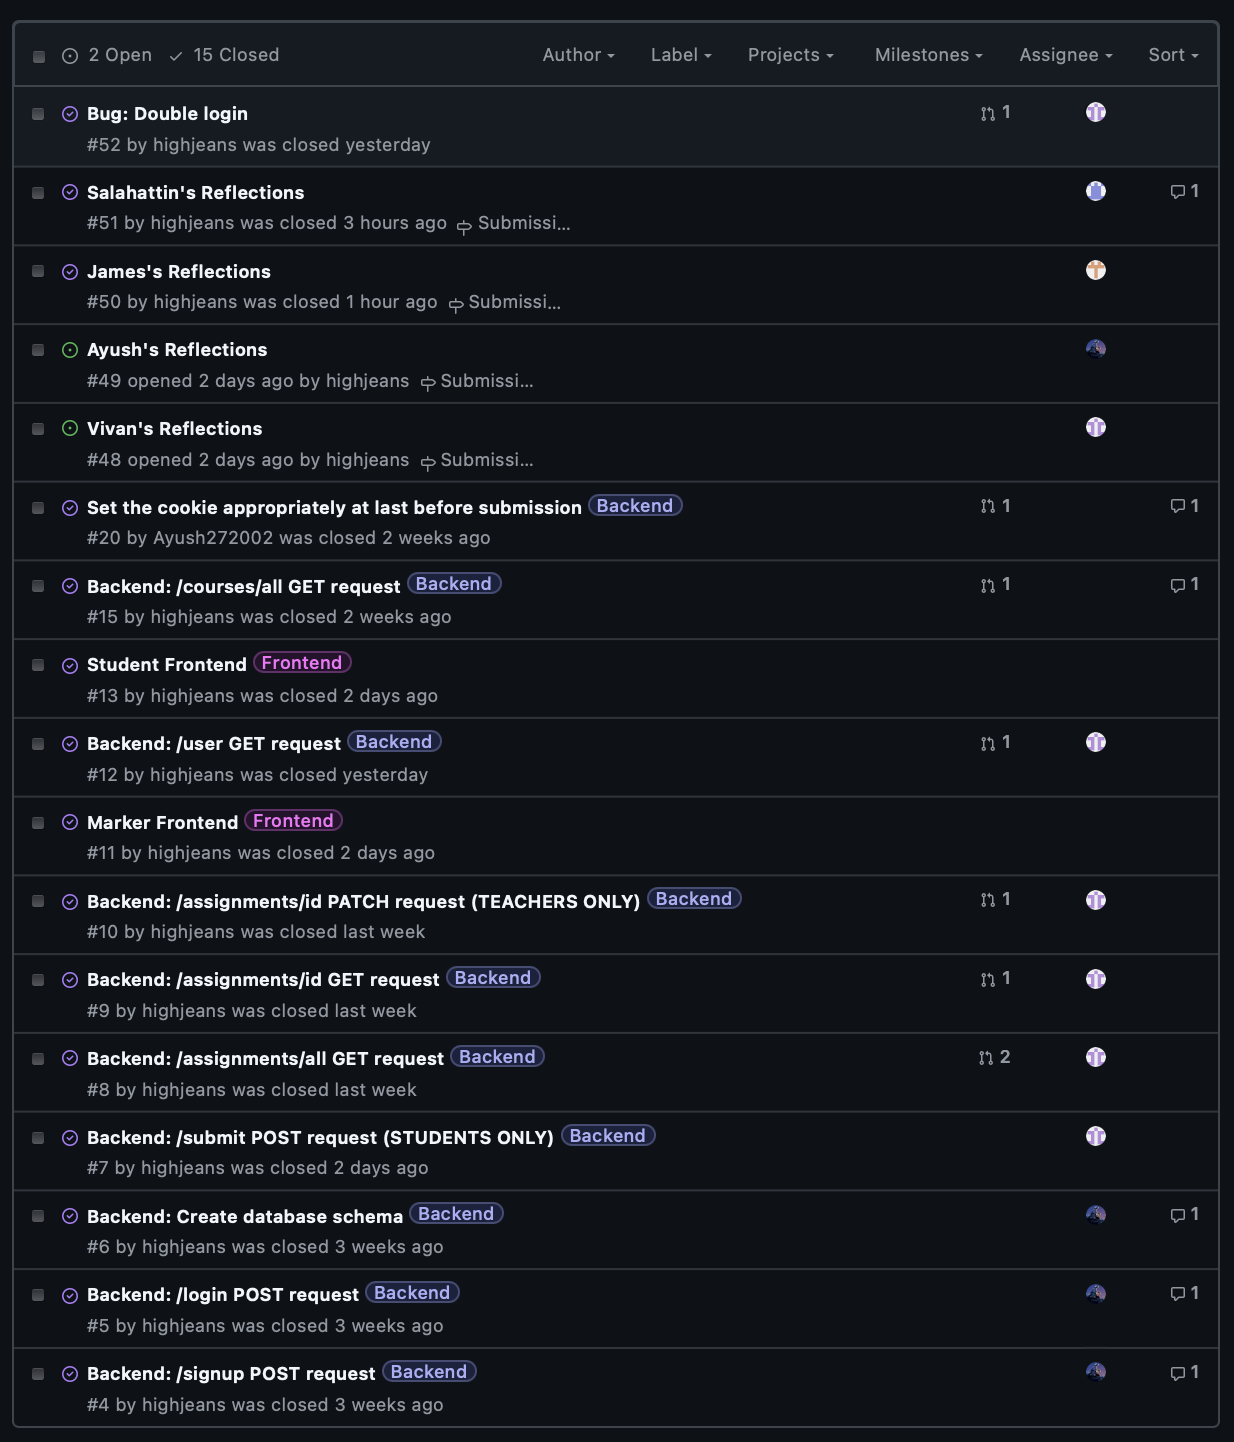
\includegraphics[width = \textwidth]{Screenshot 2024-12-10 at 21.39.08.png}
    \caption{Screenshot of all Github issues used to keep track of development}
    \label{fig:issues}
\end{figure}
\begin{figure}[H]
    \centering
    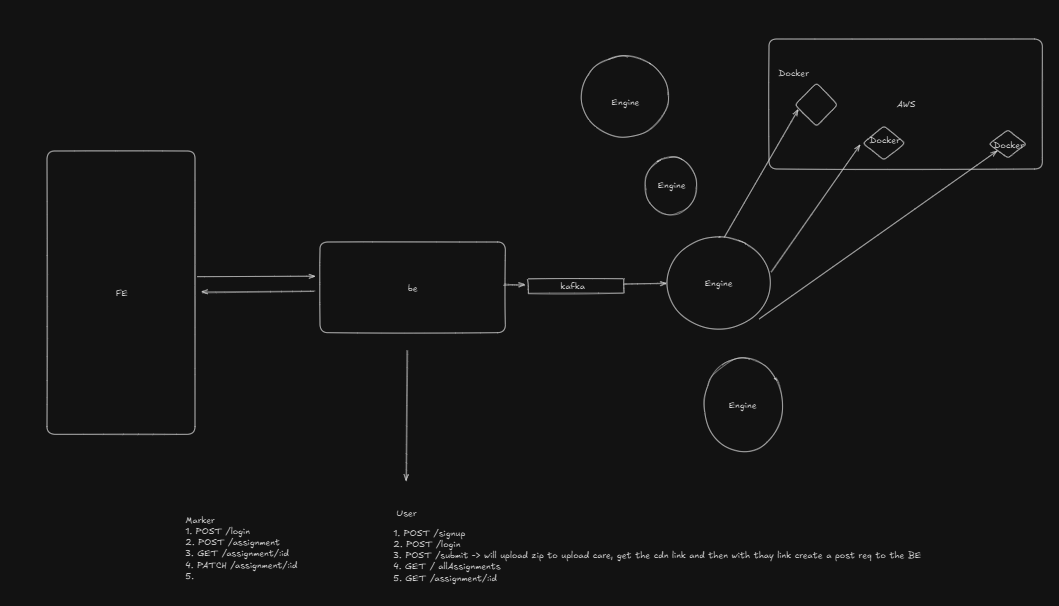
\includegraphics[width = \textwidth]{System Architecture.png}
    \caption{Screenshot of our System Architecture Design}
    \label{fig:system-architecture}
\end{figure}

\section*{Reflections}
\begin{enumerate}
    \item Vivan's Reflections
        \begin{description}
            \item[Ayush: ] % TODO
            \item[James (Ye Aung): ] % TODO
            \item[Selahattin: ] % TODO
        \end{description}
    \item Ayush's Reflections
        \begin{description}
            \item[Vivan: ] % TODO
            \item[James (Ye Aung): ] % TODO
            \item[Selahattin: ] % TODO
        \end{description}
    \item James (Ye Aung)'s Reflections
        \begin{description}
            \item[Vivan: ] Vivan’s role in our project was central to its success. He communicated expectations clearly and guided us through tasks which made everything flow seamlessly. One of his great strengths was his technical skills. He was always there and willing to help whenever the team encountered difficulties regarding the tools that we were using. He also has this unique ability to explain difficult concepts with simple easy-to-understand terms. After talking with him, difficult problems always feel manageable because he always knows which documentation to read, which problem to fix, to tackle parts of the project. This has helped me keep up with the project’s pace and allowed me to get more confident in my abilities as I worked with Next.js and backend integration. His positive attitude and reassuring explanations always make me feel at peace and not worry about the difficulties but instead guide me on how to solve the task. If there’s one area for improvement, it might be identifying potential problems earlier in the development phase to prevent last-minute fixes. That said, his contributions were invaluable and his leadership and problem-solving skills made a significant impact on my personal development throughout the project. I, along with the team, would not have done very well without his leadership and guidance.
            \item[Ayush: ] Ayush played a crucial role in our project, and he had a great impact on my learning journey. Before starting this project, I had limited experience with backend development and was new to front-end frameworks such as Next.js. This project was challenging for me, especially when it came to setting up APIs and integrating backend and frontend. Ayush was patient and he was willing to help. A lot of the time when I was stuck, I found myself seeking his guidance, and he always took the time to explain things to me thoroughly and guide me in the right direction. His support helped me overcome a lot of challenges and also made the overall process more comfortable and encouraging. He also checked up on us on our parts and offered help if we needed it. One thing I was struggling with was that he had a strict and safe deadline on our parts, and I was running late on some parts because I was studying for other modules. However, I understand that it is safer and better to complete it quickly and test for errors rather than to run late against the official deadline. It was not that much of a struggle because whenever I was running late, he stepped in to check on me and guide me.
            \item[Selahattin: ] Selahattin was responsible for designing the front end of the marker interface. Although he and I were the two less experienced members of the four, he still showed dedication and a willingness to learn. He looked up tutorials online to understand how to design and code the front end with Next.js. He also attended the group meetings regularly and wasn’t scared to ask for guidance when he was unsure about setting up APIs. I felt comfortable and motivated with him because although he and I were both inexperienced at the start of the project, he showed dedication and discipline to learn what was needed to complete his part. His positive presence and his desire to learn and grow have left a positive impact on our group’s overall performance. Another positive thing about him is that he was always on time and managed his time well on his part of the project. Although we worked together to understand the idea for both the front ends of the student and marker pages, I wish we could have coordinated more on some parts because some of our code was a bit redundant (one of us could have done it and the other could work on the next things). But overall, it turned out very well and I am grateful to have him on our team.
        \end{description}
    \item Selahattin's Reflections
        \begin{description}
            \item[Vivan: ] Vivan fostered a positive and supportive environment, making team interactions smooth and enjoyable. He wasn’t only helping me but also he was coordinating us overall, managing our chat channels and telling us exactly how to do everything and making everything run smoothly. He was quite concise and clear on what he wanted and how he wanted it. He was also well experienced in the tools we used, so he was also helping me a lot with the problems I had. He was able to break down complex technical concepts into more digestible explanations, which has helped me not feeling overwhelmed with the work we are doing. He was very active during the development process so he was very reliable whenever I was doing my work, which reduced delays which could have been caused by the issues I had. One thing he could have done can be highlighting the issues in early development so that we could have watched out for these problems, but I would say other than that he has helped me a lot with understanding NextJS and made it very easy for me to cope with the group’s expectations.
            \item[Ayush: ] For Ayush I would say working with him was really enlightening and made me learn a lot of things. Before starting this project I had very limited knowledge of backend development and not much of frontend. I started learning Next.js and API stuff specifically to use for this project so I didn’t really have prior experience on it. I was struggling a lot, especially when setting up the APIs and trying to ensure smooth integration of backend and frontend. I would say he provided very valuable guidance, patiently explaining stuff every time I was asking him to help me with the integration etc, which was almost everyday. But this level of help made understand a lot of concepts that I was struggling to understand. He has a very patient nature where he would repeat himself many times until he made sure I understood what to do which was also good for us as it formed a positive work environment where I felt really comfortable to ask questions which helped me improve a lot. One thing I would say is that he could have sent feedback more frequently on ongoing work to catch potential issues earlier and make it easy for me to work on them during the development, as when you are a beginner in the language a lot of uncertainties arise and I get overwhelmed quite easily.
            \item[James (Ye Aung): ] Working with James throughout this project was very reassuring to say the least. We had similar level of knowledge and experience, which allowed us to relate to each other’s challenges and victories easily. While I was building the marker front end for publishing assignments, viewing submissions etc he was working on student submissions the deadline for them etc. One thing I greatly appreciated was his discipline, where he was always meeting his deadlines, which also allowed both of us to meet up almost periodically to help and learn from each other as we were both beginners for NextJS stuff. He was also very keen on learning, which allowed us to work together very efficiently, as having the same mindset allowed us to develop our code quite fast. He was quite good at summarizing the issues he had and his questions so it was really easy to relay our opinions and problems with each other. Another thing I would say about him is that he sometimes overengineers solutions for some of the simpler solutions which does sometime take time, but I would say this is not a too bad quality to have overall as sometimes it does come in handy when unexpected issues arise in the code.
        \end{description}
\end{enumerate}

\end{document}
